\documentclass{article}                     % onecolumn (standard format)

\usepackage{graphicx}
\usepackage{float}
\usepackage{amsmath}
\usepackage{cite}
\usepackage{subfig}
\usepackage{rotating}
\usepackage[left=2.2cm, right=2.2cm]{geometry}
\usepackage{algpseudocode}
\usepackage{algorithm}
%\floatstyle{ruled}
\usepackage{hyperref}
\usepackage{algpseudocode}

\newfloat{algorithm}{tbp}{loa}
\providecommand{\algorithmname}{Algorithm}
\floatname{algorithm}{\protect\algorithmname}
%
% \usepackage{mathptmx}      % use Times fonts if available on your TeX system
%
% insert here the call for the packages your document requires
%\usepackage{latexsym}
% etc.
%
% please place your own definitions here and don't use \def but
% \newcommand{}{}
%

%
\begin{document}
	
	\title{Introduction to AI - assignment 2}
	
	
	\author{Oded~Yechiel         \and
		Matan~Rusanovsky
	}
	
	\date{27/11/18}
	
	\maketitle
	
	\section{Introduction}
	In this assignment we had to use the hurricane simulator from assignment 1, but operate several agents in parallel.
	
	The agents have 3 different options of operation:
	\begin{enumerate}
		\item Adversarial - where the agent must get more than the opponent.
		\item Semi-cooperative - where the agent must maximize their score.
		\item Cooperative - where the agent has to cooperate with the other agent to maximize the global score.
	\end{enumerate}
	
	\section{Base agent -- Assignment 1 recap}
	In assignment 1 a basic agent was developed, in which the method \textsc{BestAction} (In actual code you should search for \texttt{choose\_next\_action}) had to be implemented by any other inheriting agent.
	The basic agent had all of the information required by the agent to make decisions, such as the,
	\begin{itemize}
		\item current vertex
		\item number of people in the vehicle
		\item number of people saved
	\end{itemize}
	
	\section{Game tree agent}
	The three agents that are implemented in this assignment are all based on the game-tree-agent.
	\begin{algorithm}[H]
		\label{al:main}
		\caption{Game tree best action}
		\begin{algorithmic}[1]
			\Procedure{BestAction}{State, Simulator}
			\If     {\textsc{IsTerminal}(Simulator)}
			\State  \Return \textsc{NoOp()}
			\EndIf
			\State \Return \textsc{RecursiveTree}(Simulator, 0, IsZeroSumGame)
			\EndProcedure
		\end{algorithmic}
	\end{algorithm}
	The  \textsc{BestAction} function is described in Algorithm~\ref{al:main} and is fairly simple. It just checks if we are at a terminal state, and if so return a NoOp result, otherwise it starts the the recursive function described in Algorithm~\ref{al:recursive}.
	
	The terminal state, shown in Algorithm~\ref{al:terminal}, is a boolean function. It returns true if the time surpassed the deadline, or if there are no more people to save. 
	

	
	\begin{algorithm}
		\caption{Terminal position}
		\label{al:terminal}		
		\begin{algorithmic}[1]
			\Procedure{IsTerminal}{Simulator}
			\If     {Simulator.Time $ \geq $ Simulator.Deadline}
			\State  \Return True
			\ElsIf     {Simulator.PeopleInTowns == 0 and $ \forall agent \quad agent.carrying == 0 $}
			\State  \Return True
			\Else
			\State \Return False
			\EndIf
			\EndProcedure
		\end{algorithmic}
	\end{algorithm}
	
	The recursive tree function in Algorithm~\ref{al:recursive} receives a simulator, that hold all of the data and used to emulate each action, depth value representing the depth of tree, and a Boolean stating whether it is a zeros sum game. 
	
	The algorithm starts by checking for terminal states and checks if the depth is maxed out for cutoff purposes. For terminal states the actual value, i.e., number of people saved, of each agent is returned. Maxing out depth returns a heuristic (line~\ref{al:h}) of how many people each agent may save, disregarding the other agent and assuming each town with people is the only town with people.
	This same heuristic was used in assignment 1.
	
	The function continues, if not returned, to a for loop (line \ref{al:actions}) that branches every possible action of an agent, and calls recursively to itself with an emulated simulator where its the next agent's turn, and depth is increased by 1. 
	
	The result of this action is compared with all of the other actions and the best action's value is returned if the depth is larger than 0, otherwise the best action itself.
	For each type of agent (adversarial, cooperative, semi-cooperative) the comparison function is different and will be elaborated in the following section.
	
	In case the game is adversarial, or a zero sum game, an alpha-beta cutoff is also compared to try and trim branches off.
	
	\begin{algorithm}[H]
		\label{al:recursive}
		\caption{Game tree recursive tree expansion}
		\begin{algorithmic}[1]
			\Procedure{RecursiveTree}{Simulator, Depth, IsZeroSumGame}
	       \If {\textsc{IsTerminal}(Simulator)}
	       \State \Return \textsc{Value}(Simulator)
	       \EndIf
	       \If {Depth reached MAX\_DEPTH:}
	       \State \Return \textsc{Heuristic}(Simulator) \label{al:h}
			\EndIf
			
			\State BestValue $\longleftarrow  [-inf, -inf] $
			
			\State BestMove  $\longleftarrow -1 $
			
			\For {each Action $ \in $ possible actions of current player}\label{al:actions}
			
				\State Simulator.\textsc{EmulateAction}(Action)
				
				\State NewValue $ \leftarrow $ \textsc{RecursiveTree}(Simulator, Depth+1, IsZeroSumGame)
				
				\If {\textsc{IsBetterAction}(NewValue, BestValue)} \label{al:is_better}
				
				\State BestValue $ \longleftarrow $ NewValue
				
				\State BestMove $ \longleftarrow $ Action
				\EndIf
				
				\If {IsZeroSumGame is True} \label{al:alphabeta}
				
				\EndIf
				
			\EndFor
			
			\If {Depth == 0}
			
				\Return BestMove
				
			\Else
			
				\Return BestValue
				
			\EndIf
			\EndProcedure
		\end{algorithmic}

	\end{algorithm}
			
	\subsection{Adversarial agent}
	The adversarial agent is a zero sum game agent. In plain words, the agent prefers that everyone will die as long as the opponent agent will not save more people than him.
	
	Therefore, the \textsc{IsBetterAction} shown in Algorithm~\ref{al:recursive} in line~\ref{al:is_better} will be as follows:
	\begin{algorithm}[H]
		\label{al:adv}
		\caption{Adversarial action assessment}
		\begin{algorithmic}[1]
			\Procedure{IsBetterAction}(NewValue, BestValue)
			\State $ Best \leftarrow BestValue[CurrentAgent] - BestValue[OtherAgent]$
			\State $ New \leftarrow NewValue[CurrentAgent] - NewValue[OtherAgent]  $
			\If     {$ New > Best $}
			\State  \Return True
			\Else   \Return False
			\EndIf
			\EndProcedure
		\end{algorithmic}
	\end{algorithm}
	
	The action is better than other options in the case where the difference in values is higher than previous difference in value. 


	\subsection{semi-cooperative agent}
	The semi-cooperative agent tries to maximize its own value, disregarding the other agent value. This is partially true, the agent will help the other agent if he does not sacrifice his own score.
	The \textsc{IsBetterAction} will be as follows:
	
	\begin{algorithm}[H]
		\label{al:coop}
		\caption{Semi-cooperative action assessment}
		\begin{algorithmic}[1]
			\Procedure{IsBetterAction}(NewValue, BestValue)
			\State $ Best \leftarrow BestValue[CurrentAgent]$
			\State $ New \leftarrow NewValue[CurrentAgent]$
			\If     {$ New > Best~or~(New == Best~and~NewValue[OtherAgent] > BestValue[OtherAgent])$}
			\State  \Return True
			\Else   \Return False
			\EndIf
			\EndProcedure
		\end{algorithmic}
	\end{algorithm}

	
	\subsection{Cooperative agent}
	
	The cooperative agent tries to maximize the global score, sacrificing his own score for the good of the team. 
	The \textsc{IsBetterAction} will be as follows:
	\begin{algorithm}[H]
		\label{al:semi}
		\caption{Cooperative action assessment}
		\begin{algorithmic}[1]
			\Procedure{IsBetterAction}(NewValue, BestValue)
			\State $ Best \leftarrow BestValue[CurrentAgent] + BestValue[OtherAgent]$
			\State $ New \leftarrow NewValue[CurrentAgent] + NewValue[OtherAgent]  $
			\If     {$ New > Best $}
			\State  \Return True
			\Else   \Return False
			\EndIf
			\EndProcedure
		\end{algorithmic}
	\end{algorithm}

	
	\section{Example}
	Fig.~\ref{fig:worlddrawing} shows a world where there are 5 vertices. There are people in vertices, V1, V4, and V5 with 1, 2, and 2 people respectively. There are shelters in vertices V0 and V3. Agent0 start at V0. Agent1 starts at V4 and immediately pick up the people there. The deadline is in 16[time].
	\begin{figure}
		\centering
		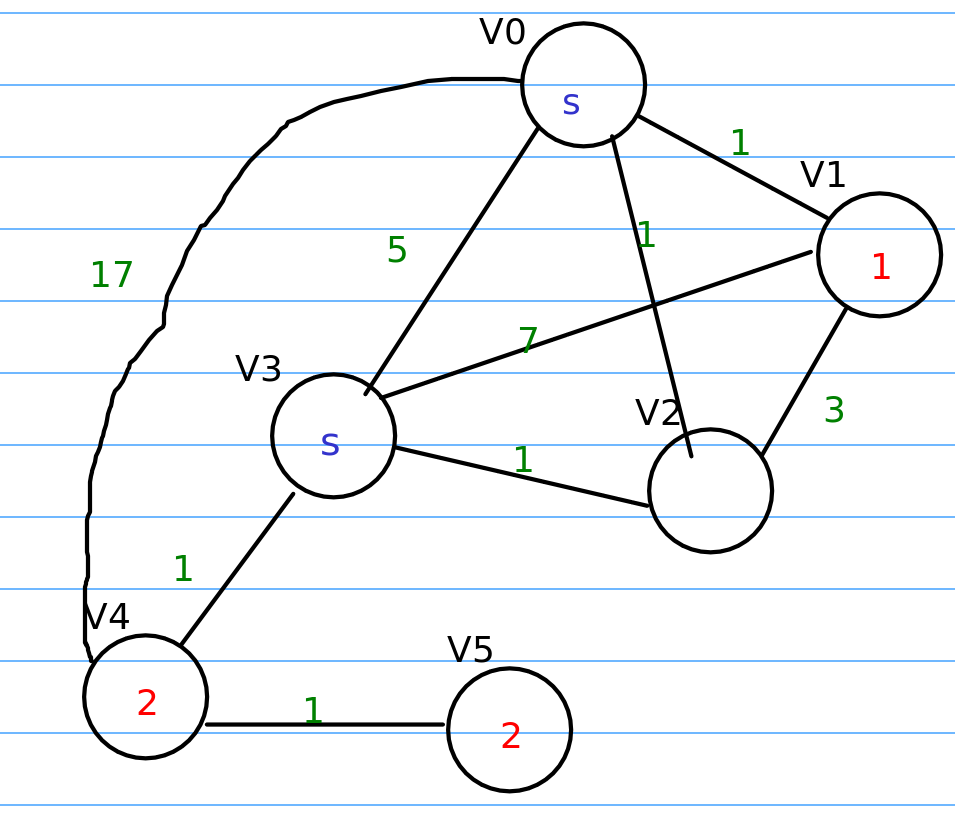
\includegraphics[width=0.5\linewidth]{world_drawing}
		\caption{An example of a world where Agent0 will choose a different option per type of game. Agent1 starts at V0. Agent 2 starts at V4 and immediately picks up the 2 people.}
		\label{fig:worlddrawing}
	\end{figure}

	\begin{itemize}
		\item Adversarial agent
		
		It is clear that agent0 has to go to V4, thus finishing the game with 0 people saved for each agent. Otherwise, agent1 will reach a shelter and rescue 2 people.
		
		\item Semi-cooperative agent
		
		Agent0 will go to V1 picking up the person and will go back to V0 maximizing the amount of people he could save. Agent1 will go immediately to V3 saving the 2 people he is carrying, as there is no time to go to V5.
		
		\item Fully cooperative agent
		
		Agent0 will go to V2 in order to conserve as much time as he can so agent1 will reach V5 and save 1 more person. Agent0 is sacrificing his score for the greater good.
		
	\end{itemize}
\end{document}

